Решается задача оптимизации гиперпараметров модели глубокого обучения. Для оптимизации гиперпараметров модели предлагаются алгоритмы, основанные на градиентном спуске. Так как сложность рассматриваемых алгоритмах сопоставима со сложностью оптимизации параметров модели, предлагается оптимизировать параметры и гиперпараметры в единой процедуре. Для выбора адекватных значений гиперпараметров вводятся вероятностные предположения о распределении параметров. В качестве оптимизируемой функции выступает байесовская обоснованность модели и кросс-валидация. Для получения оценки обоснованности используются вариационные методы. Проводится вычислительный эксперимент на нескольких выборках.

Одна из проблем построения моделей глубокого обучения --- большое число параметров модели~\cite{hinton_rbm}, которое достигает нескольких миллионов, а оптимизация модели достигает десятков дней~\cite{suts}. Задача выбора модели глубокого обучения включает в себя выбор стратегии построения модели, эффективной по вычислительным ресурсам. Проблема оптимизации параметров модели глубокого обучения является вычислительно сложной в силу невыпуклости оптимизируемой функции потерь. Поэтому задача поиска параметров оптимизации является важной, и нахождение оптимальныых гиперпараметров сильно влияет на итоговое качество модели. 

В данной работе сравниваются градиентные методы оптимизации гиперпараметров. Основным достоинством подобных алгоритмов является их возможность одновременной оптимизации значительного числа гиперпараметров. В качестве базового алгоритма выступает алгоритм выбора гиперпараметров модели с использованием случайного поиска.  В работах\cite{hyper_mad,hyper_hoag,greed_hyper} в качестве целевой функции потерь рассматривается потеря на валидационной подвыборке с $L_2$ регуляризацией. В данной работе рассматривается общая задачи оптимизации гиперпараметров. Рассматриваеые алгоритмы и целевые функции потерь реализованы и представлены в качестве библиотеки для оптимизации гиперпараметров моделей~\cite{pyfos}. Основным теоретическим вкладом данной главы является анализ рассматриваемых алгоритмов оптимизации гиперпараметров при использовании функции потерь общего вида, а также исследование качества и устойчивости итоговых моделей в случае использования кросс-валидации и вариационной оценки обоснованности.  В экспериментальной части в качестве критерия выбора модели выступают вариационная нижняя оценка обоснованности модели и ошибка на валидационной части выборки. В отличие от~\cite{hyper_hoag}, где также производится сравнение алгоритмов оптимизации гиперпараметров, в данной работе исследуется поведение алгоритмов на выборках большой мощности, таких как WISDM~\cite{wisdm} и MNIST~\cite{mnist}.
Численные эксперименты показывают, что при значительном количестве гиперпараметров, сопоставимым с количеством параметров модели, рассматриваемые алгоритмы предпочтительнее стохастических. 




\section{Постановка задачи оптимизации гиперпараметров моделей}
Пусть задана дифференцируемая по параметрам модель, приближающая зависимую переменную~$y$:
\[
	\mathbf{f}(\mathbf{w}, \mathbf{x}):\mathbb{W} \times \mathbb{X} \to \mathbb{Y}, \quad \mathbf{w} \in \mathbb{W}.
\]
Как и в предыдущем разделе, будем полагать, что структура модели $\boldsymbol{\Gamma}$ для вероятностной модели глубокого обучения $\mathbf{f}$ определена однозначно и метапараметры $\lam$ определены однозначно:
\[
    \prior = p(\w,\G|\h), \quad \priorw = p(\w|\h),\quad    \LL = p(\y|\X,\w).
\]

Пусть априорное распределение параметров имеет вид
\begin{equation}
\label{eq:prior}
	\mathbf{w} \sim \mathcal{N}(\mathbf{0}, \mathbf{A}^{-1}),
\end{equation}
где $\mathbf{A}^{-1} = \text{diag}[\alpha_1, \dots, \alpha_u]^{-1}$ --- матрица ковариаций диагонального вида.


Задача оптимизации гиперпараметров зависит как от критерия выбора модели, так и от метода оптимизации параметров модели.
Проиллюстрируем задачу оптимизации гиперпараметров \textit{двусвзяным байесовским выводом}.

\begin{example}
Для дальнейшей формализации задачи в общем виде переобозначим
\begin{equation}
\label{eq:bayes0}
	\boldsymbol{\theta} = \mathbf{w}, \quad \mathbf{h} = [\alpha_1, \dots, \alpha_u],	
\end{equation}
где $\boldsymbol{\theta}$ --- множество оптимизируемых параметров модели, $\mathbf{h}$ --- множество гиперпараметров модели.

На \textit{первом уровне} байесовского вывода производится оптимизация параметров~\eqref{eq:posterior} модели $\mathbf{f}$ по заданной выборке $\mathfrak{D}$:
\begin{equation}
\label{eq:bayes1}
{\boldsymbol{\theta}}^{*} = \argmax \bigl(-L\bigr) = p(\mathbf{w}|\mathbf{X}, \mathbf{y}, \mathbf{h}) = \frac{p(\mathbf{y}|\mathbf{X},\mathbf{w})p(\mathbf{w}|\mathbf{h})}{p(\mathbf{y}|\mathbf{X},\mathbf{h})}.
\end{equation}

На \textit{втором уровне} производится оптимизация апостериорного распределения гиперпараметров $\mathbf{h}$:
\[
p(\mathbf{h}|\mathbf{X}, \mathbf{y}) \propto p(\mathbf{y}|\mathbf{X},\mathbf{h})p(\mathbf{h}),
\]
где знак <<$\propto$>> означает равенство с точностью до нормирующего множителя.

Полагая распределение параметров $p(\mathbf{h})$ равномерным на некоторой большой окрестности, получим задачу оптимизации гиперпараметров:
\begin{equation}
\label{eq:bayes2}
	p(\mathbf{y}|\mathbf{X},\mathbf{h}) = \int_{\mathbf{w} \in \mathbb{R}^u} p(\mathbf{y}|\mathbf{X}, \mathbf{w}) p(\mathbf{w}|\mathbf{h}) = -Q \to \max_{[\alpha_1, \dots, \alpha_n] \in \mathbb{R}^{n}}.
\end{equation}
\end{example}

Как и в общей задаче~\eqref{eq:optim_problem},\eqref{eq:hyper_optim}, 
требуется найти параметры ${\boldsymbol{\theta}}^{*}$ и гиперпараметры $\mathbf{h}^{*}$ модели, доставляющие минимум следующей функции:
\begin{equation}
\label{eq:main}
    \mathbf{h}^{*} = \argmin_{\mathbf{h} \in \mathbb{H}} Q(\mathbf{h}|  \boldsymbol{\theta}^{*}, \mathbf{X}, \mathbf{y} ),
\end{equation}
\begin{equation}
\label{eq:main2}
	\boldsymbol{\theta}^{*}(\mathbf{h}) =  \argmin_{\boldsymbol{\theta} \in \mathbb{R}^u} L(\boldsymbol{\theta}|  \mathbf{h},  \mathbf{X}, \mathbf{y}),
\end{equation}
где $L,Q$ --- функции потерь и валидации (см. Опр.~\ref{def:l},\ref{def:q}).

Рассмотрим вид переменной $\boldsymbol{\theta}$ и функций $L, Q$ для различных методов выбора модели и оптимизации ее параметров.

\textbf{Базовый метод. }
Пусть оптимизация параметров и гиперпараметров производится по всей выборке $\mathfrak{D}$ по одной и той же функции $L=Q$:
$$L(\boldsymbol{\theta}|  \mathbf{h},  \mathbf{X}, \mathbf{y}) = Q(\mathbf{h}|  \boldsymbol{\theta}, \mathbf{X}, \mathbf{y} ) = -\text{log}p(\mathbf{y}, \mathbf{w} | \mathbf{X}, \mathbf{h}) = \text{log} p(\mathbf{y}|\mathbf{X}, \mathbf{w})+\text{log}p(\mathbf{w}|\mathbf{h})$$.

Вариационным параметрам $\boldsymbol{\theta}$ модели $\mathbf{f}$  соответствует вектор параметров модели: 
\[
\boldsymbol{\theta} = \mathbf{w}.
\]

\textbf{Кросс-валидация. }
Разобьем выборку $\mathfrak{D}$ случайно на $K$ равных частей:
\[
\mathfrak{D} = \mathfrak{D}_1 \sqcup \dots \sqcup \mathfrak{D}_k, \mathfrak{D}_k = \{\mathbf{X}_k, \mathbf{y}_k\}, \quad k=1,\dots,K.
\]


Запустим $K$ оптимизаций модели, каждую на своей части выборки. Положим $\boldsymbol{\theta} = [\mathbf{w}_1, \dots, \mathbf{w}_K]$, где $\mathbf{w}_1, \dots, \mathbf{w}_K$ --- параметры модели при оптимизациях $1, \dots, K$.
 
Положим функцию $L$ равной  среднему значению минус логарифма апостериорной вероятности по всем $k-1$ разбиениям $\mathfrak{D}$:
\begin{equation}
L = -\frac{1}{K}\sum_{k=1}^K \bigl(\frac{K}{K-1}\text{log}p(\mathbf{y}_k|\mathbf{X}_k, \mathbf{w}_k) + \text{log}p(\mathbf{w}_k|\mathbf{h})\bigr).
\label{eq:cv}
\end{equation}

Положим функцию $Q$ равной минус среднему значению правдоподобия выборки по частям выборки $\mathfrak{D}_k$, на которых не проходила оптимизация параметров:
\[
Q = -\frac{1}{k}\sum_{q=1}^k k\text{log}p(\mathbf{y} \setminus \mathbf{y}_k|\mathbf{X}_k \setminus \mathbf{X}, \mathbf{w}_q).
\]
где операция <<$\mathbf{X} \setminus \mathbf{X}_k$>> определяется как взятие описаний всех объектов $\mathbf{X}$ за исключением описаний объектов из $\mathbf{X}_k$.


\textbf{Вариационная оценка обоснованности. }
Положим $L=Q$, равной вариационной оценке обоснованности модели:
\begin{equation} 
\text{log}~p(\mathbf{y}|\mathbf{X},\mathbf{h})  
\geq 
-\text{D}_\text{KL} \bigl(q(\mathbf{w})||p(\mathbf{w}|\mathbf{h})\bigr) + \int_{\mathbf{w}} q(\mathbf{w})\text{log}~{p(\mathbf{y}|\mathbf{X},\mathbf{w},\mathbf{h})} d \mathbf{w}  \approx
\label{eq:hyper_elbo}
\end{equation}
\[
\approx \sum_{i=1}^m \text{log}~p({y}_i|\mathbf{x}_i, \mathbf{w}_i) - D_\text{KL}\bigl(q (\mathbf{w}) || p (\mathbf{w}|\mathbf{h})\bigr) = -L = -Q,
\]
где $q$ --- нормальное распределение с диагональной матрицей ковариаций:
\begin{equation}
	q \sim \mathcal{N}(\boldsymbol{\mu}_q, \mathbf{A}^{-1}_q),
\label{eq:diag}
\end{equation}
где $\mathbf{A}_q = \text{diag}[\alpha^q_1, \dots, \alpha^q_u]^{-1}$ --- диагональная матрица ковариаций, $\boldsymbol{\mu}_q$ --- вектор средних компонент.
Расстояние $D_\text{KL}$ между двумя гауссовыми величинами задается как 
\[
	D_\text{KL}\bigl(q (\mathbf{w}) || p (\mathbf{w}|\mathbf{h})\bigr) = \frac{1}{2} \bigl( \text{Tr} [\mathbf{A}\mathbf{A}^{-1}_q] + (\boldsymbol{\mu} - \boldsymbol{\mu}_q)^\mathsf{T}\mathbf{A}(\boldsymbol{\mu} - \boldsymbol{\mu}_q) - u +\text{ln}~|\mathbf{A}^{-1}| - \text{ln}~|\mathbf{A}_q^{-1}| \bigr).
\]
В качестве вариационных параметров $\boldsymbol{\theta}$ выступают параметры распределения $q$:
\[
\boldsymbol{\theta} = [\alpha_1, \dots, \alpha_u, {\mu}_1,\dots,{\mu}_u].
\]




\section{Градиентные методы оптимизации гиперпараметров}
В данном разделе приводится описание рассматриваемых градиентных методов.
Краткая характеристика и основные преимущества каждого из представленных методов отображены в Табл.~\ref{table:algo_descr},~\ref{table:algo_descr2}.



\begin{table}[H]
\small
% Алгоритм & Тип алгоритм & Время & Плюсы & Минусы 

\begin{tabularx}{\textwidth}{|X|X|X|X|}
\hline
\bf Алгоритм & \bf Тип алгоритма & \bf Преимущества алгоритма & \bf Недостатки алгоритма  \\ 
Случайный поиск & стохастический & простота реализации& Алгоритм неэффективен при большом количестве гиперпараметров (проклятие размерности)  \\ \hline
Жадный алгоритм~\cite{greed_hyper} & градиентный & Возможность одновременной оптимизации параметров и гиперпараметров & Жадность алгоритма \\ \hline
HOAG~\cite{hyper_hoag} & градиентный & Быстрая сходимость & Алгоритм требователен к настройкам параметров \\ \hline 
DrMAD~\cite{hyper_mad} & градиентный & Алгоритм учитывает алгоритм оптимизации параметров модели и его параметры & Алгоритм страдает от проблем неустойчиовтси градиентного спуска (градиентный взрыв и затухание); Алгоритм работает в очень жетских предположениях. \\ \hline
\end{tabularx}

\caption{Преимщуества и недостатки рассматриваемых алгоритмов}
\label{table:algo_descr}

\end{table}


\begin{table}[H]
\small
% Алгоритм & Тип алгоритм & Время & Плюсы & Минусы 

\begin{tabularx}{\textwidth}{|X|X|X|X|}
\hline
\bf Алгоритм & \bf Тип & \bf Сложность итерации оптимизации & \bf Предположения \\ 
\hline
Случайный поиск & стохастический & $O(\eta s |\hat{\mathfrak{D}}|)$& -  \\ \hline
Жадный алгоритм~\cite{greed_hyper} & градиентный & $O(\eta (s+h) |\hat{\mathfrak{D}}|)$ & $\mathbf{H}(\boldsymbol{\theta}) = \mathbf{I}$  \\ \hline
HOAG~\cite{hyper_hoag} & градиентный & $O(\eta s |\hat{\mathfrak{D}}| + h^2 |\hat{\mathfrak{D}}| + \text{o}),$ где $o$ ---сложность решения системы линейных уравнений& первая производная $Q$  и вторая производная $L$  являются липшецевыми функциями  $\text{det}\mathbf{H} \neq \mathbf{0}$;  \\ \hline
DrMAD~\cite{hyper_mad} & градиентный &$O(\eta s |\hat{\mathfrak{D}}|)$ & Траектория оптимизации вариационных параметров $\boldsymbol{\theta}$ = $\boldsymbol{\theta}^0, \dots \boldsymbol{\theta}^\eta$  линейна \\ \hline
\end{tabularx}

\caption{Сложность и предположения для различных алгоритмов оптимизации гиперпараметров}
\label{table:algo_descr2}

\end{table}






Рассмотрим случай, когда оптимизация~\eqref{eq:main2} параметров $\boldsymbol{\theta}$ производится с использованием градиентных методов.  Пусть задан оператор стохастического градиентного спуска $T$~\eqref{eq:sgd_operator}, оптимизирующий вариационные параметры $\boldsymbol{\theta}$.
Пусть оператор $T$ производит $\eta$ шагов оптимизации:
\begin{equation}
\label{eq:gd}
	 \boldsymbol{\theta}^{*} = T \circ T \circ \dots \circ T(\boldsymbol{\theta}^{0} | L, \mathbf{y}, \mathbf{X}, \mathbf{h}, \boldsymbol{\lambda}) = T^\eta(\boldsymbol{\theta}^{0} | L, \mathbf{y}, \mathbf{X}, \mathbf{h}, \boldsymbol{\lambda}),
\end{equation}
где 
$$
	T( \boldsymbol{\theta}| L,\mathbf{X},  \mathbf{y},  \mathbf{h}, \boldsymbol{\lambda}) = \boldsymbol{\theta} - \lambda_{\text{lr}} \nabla L(\boldsymbol{\theta}|   \mathbf{h},  \hat{\mathbf{X}}, \hat{\mathbf{y}}), 
$$
$ \lambda_{\text{lr}}$ --- длина шага градиентного спуска, $\boldsymbol{\theta}^0$ --- начальное значение параметров $\boldsymbol{\theta}$, $\hat{\mathbf{y}}, \hat{\mathbf{X}}$ --- случайная подвыборка заданной мощности выборки $\mathfrak{D}$. В данной работе в качестве опреатора оптимизации параметров модели выступает стохастический градиентный спуск~\eqref{eq:sgd_operator}.

Перепишем задачу оптимизации~\eqref{eq:main}, ~\eqref{eq:main2} в следующем виде
\begin{equation}
\label{eq:hyper_optim}
    \mathbf{h}^{*} = \argmax_{\mathbf{h} \in \mathbb{R}^h} Q(T^\eta(\boldsymbol{\theta} | L, \mathbf{y}, \mathbf{X}, \mathbf{h}, \boldsymbol{\lambda})),
\end{equation}
где $\boldsymbol{\theta}^0$ --- начальное значение параметров $\boldsymbol{\theta}$.
В дальнейшем для удобства будем применять сокращенные формы $Q(\mathbf{h}| \boldsymbol{\theta}), L(\boldsymbol{\theta}| \mathbf{h}), T(\boldsymbol{\theta}, \mathbf{h}).$

Оптимизационную задачу~\eqref{eq:hyper_optim} предлагается решать с использованием градиентного спуска. Вычисление градиента от функции $Q( T^\eta(\boldsymbol{\theta}_0| \mathbf{h}))$ по гиперпараметрам $\mathbf{h}$ является вычислительно сложным в силу внутренней процедуры оптимизации $\boldsymbol{\theta}^{*} = T(\boldsymbol{\theta}_0, \mathbf{h})$. 
Общая схема  оптимизации гиперпараметров представлена следующим образом:
\begin{enumerate}
\item От 1 до  $l$:
\item Инициализировать парметры $\boldsymbol{\theta}$ при условии гиперпараметров $\mathbf{h}$.
\item Приближенно решить задачу оптимизации~\eqref{eq:hyper_optim} и получить новый вектор параметров $\mathbf{h}'$
\item $\mathbf{h} = \mathbf{h}'$.
\end{enumerate}
Здесь $l$ --- число итераций оптимизации гиперпараметров. Рассмотрим методы приближенного решения данной задачи оптимизации.
Псевдокод общего алгоритма оптимизации гиперпараметров приведен на Рис.~\ref{alg:hyperparam_optim}.


\textbf{Жадный алгоритм. }
В качестве  правила обновления вектора гиперпараметров $\mathbf{h}$ на каждом шаге оптимизации~\eqref{eq:gd} выступает градиентный спуск с учетом обновления параметров $\boldsymbol{\theta}$ на данном шаге:
\begin{equation}
\label{eq:greed}
\mathbf{h}' =	 \mathbf{h} -  \lambda_{\text{lr}}^{\mathbf{h}} \nabla_{\mathbf{h}}  Q \bigl(\mathbf{h}, T(\boldsymbol{\theta}^{0}, \mathbf{h})\bigr) = \mathbf{h} -  \lambda_{\text{lr}}^{\mathbf{h}} \nabla_{\mathbf{h}}  Q\bigl(\mathbf{h}, \boldsymbol{\theta} -  \lambda_{\text{lr}} \nabla L(\boldsymbol{\theta}| \mathbf{h})\bigr),
\end{equation}
где $ \lambda_{\text{lr}}^{\mathbf{h}}$ --- длина шага оптимизации гиперпараметров.
Псевдокод жадного алгоритма оптимизации гиперпараметров приведен на Рис.~\ref{alg:greedy}.

\textbf{Алгоритм HOAG. }
Предлагается получить приближенное значения градиента гиперпараметров $\nabla_{\mathbf{h}} Q \bigl(\mathbf{h}, T^\eta(\boldsymbol{\theta}^0)\bigr)$ на основе следующей формулы:
\[
\nabla_{\mathbf{h}} Q \bigl(T^\eta(\boldsymbol{\theta}^0, \mathbf{h})\bigr) = \nabla_{\mathbf{h}} Q( \mathbf{h}| \boldsymbol{\theta}) - (\nabla^2_{\boldsymbol{\theta}, \mathbf{h}} L(\boldsymbol{\theta}| \mathbf{h}))^\text{T}\mathbf{H}(\boldsymbol{\theta})^{-1}\nabla_{\boldsymbol{\theta}} Q( \mathbf{h}| \boldsymbol{\theta}),
\]
где $\mathbf{H}$ --- гессиан функции $L$ по вариационным параметрам $\boldsymbol{\theta}$.

Процедура получения приближенного значения градиента гиперпараметров $\nabla_{\mathbf{h}} Q$  производится итеративно.
\begin{enumerate}
\item Провести $\eta$ шагов оптимизации: $\boldsymbol{\theta} = T(\boldsymbol{\theta}_0, \mathbf{h})$.
\item Решить линейную систему для вектора $\boldsymbol{\lambda}$: $\mathbf{H}(\boldsymbol{\theta})\boldsymbol{\lambda} =  \nabla_{\boldsymbol{\theta}} Q(\boldsymbol{\theta}| \mathbf{h})$.
\item Приближенное значение градиентов гиперпараметра вычисляется как $\hat{\nabla}_{\mathbf{h}}Q = \nabla_{\mathbf{h}}Q(\boldsymbol{\theta}| \mathbf{h}) -\nabla_{\boldsymbol{\theta}, \mathbf{h}} L(\boldsymbol{\theta}| \mathbf{h})^T\boldsymbol{\lambda}$.
\end{enumerate}

Итоговое правило обновления:
\begin{equation}
\label{eq:update_hyper}
\mathbf{h}' = \mathbf{h} -  \lambda_{\text{lr}}^{\mathbf{h}} \hat{\nabla}_{\mathbf{h}}Q.
\end{equation}

В данной работе для приближенного решения  шага 2 алгоритма HOAG используется стохастический градиентный спуск в силу сложности вычисления гессиана $\mathbf{H}(\boldsymbol{\theta})$.
Псевдокод алгоритма HOAG приведен на Рис.~\ref{alg:hoag}.

\textbf{Алгоритм DrMad. }
TODO: доказать корректность?
Для получения градиента от оптимизируемой функции $Q$ как от функции от начальных параметров $\boldsymbol{\theta}^0$ предлагаетя пошагово восстановить $\eta$ шагов оптимизации $T(\boldsymbol{\theta}^0)$ в обратном порядке аналогично методу обратного распространения ошибок. Для упрощения данной процедуры вводится предположение,что траектория изменения параметров $\boldsymbol{\theta}$ линейна:
\begin{equation}
\label{eq:mad_lin}
\boldsymbol{\theta}^\tau = \boldsymbol{\theta}^0 + \frac{\tau}{\eta} (T(\boldsymbol{\theta})- \boldsymbol{\theta}^0).
\end{equation}

Алгоритм вычисления приближенного значения градиента $\nabla \mathbf{h}$ является частным случаем алгоритма обратного распространения ошибки и представим в следующем виде:
\begin{enumerate}
\item Провести $\eta$ шагов оптимизации: $\boldsymbol{\theta} = T(\boldsymbol{\theta}_0, \mathbf{h})$.
\item Положим $\hat{\nabla} \mathbf{h} = \nabla_\mathbf{h} Q( \mathbf{h}, \boldsymbol{\theta}).$ 
\item Положим $d\mathbf{v} = \mathbf{0}.$
\item Для $\tau = \eta \dots 1 $ повторить:
\item Вычислить значения параметров $\boldsymbol{\theta}^\tau$\eqref{eq:mad_lin}.
\item $d\mathbf{v} =   \lambda_{\text{lr}} \hat{\nabla}_{\boldsymbol{\theta}}$.
\item $\hat{\nabla} \mathbf{h} =  \hat{\nabla} \mathbf{h} - d\mathbf{v}\nabla_{\mathbf{h}} \nabla_{\boldsymbol{\theta}} Q$.
\item $\hat{\nabla} \boldsymbol{\theta}  = \hat{\nabla} \boldsymbol{\theta}  - d\mathbf{v}\nabla_{\boldsymbol{\theta}} \nabla_{\boldsymbol{\theta}} Q$.
\end{enumerate}

Итоговое правило обновления гиперпараметров аналогично~\eqref{eq:update_hyper}.
Псевдокод общего алгоритма оптимизации гиперпараметров приведен на Рис.~\ref{alg:drmad}.

В работе~\cite{hyper_mad} отмечается неустойчивость алгоритма при высоких значениях длины шага градиентного спуска $ \lambda_{\text{lr}}$. Поэтому вместо исходного правила~\eqref{eq:mad_lin} в данной работе первые 5\% значений параметров не рассматриваются, а также учитывается только каждый $\tau_k$ шаг оптимизации:
\begin{equation}
\label{eq:mad_lin2}
\boldsymbol{\theta}^\tau = \boldsymbol{\theta}^{\tau_0} + \frac{\tau}{\eta} (T(\boldsymbol{\theta})-\boldsymbol{\theta}^{\tau_0}), \quad \tau \in \{\tau_0,\dots,\eta\}, \tau \text{ mod } \tau_k = 0,
\end{equation}
где $\tau_0 = [0.05 \cdot \eta]$.

Иллюстративный пример поведения представленных методов представлен на Рис.~\ref{fig:traj}. Жадный алгоритм, соответствющий красной линии на графике, оптимизирует гиперпараметры во время процедуры оптимизация вариационных параметров $\boldsymbol{\theta}$. Алгоритм HOAG оптимизирует гиперпараметры после каждой процедуры оптимизации вариационных параметров. Алгоритм DrMAD использует линеаризованную аппроксимацию траектории оптимизации вариационных параметров $\boldsymbol{\theta}$. 

\begin{figure}
%GENERAL
    \begin{algorithmic}[1]
\REQUIRE $\mathbf{X}, \mathbf{y}, p(\mathbf{w}|\mathbf{h}), \boldsymbol{\theta}^0$;
\REQUIRE количество итераций $l$ градиентной оптимизации гиперпараметров; 
\REQUIRE количество итераций $\eta$ оптимизации вариационных параметров;
\ENSURE оптимальные значения параметров $\mathbf{h}$;
\FOR{$r=1,\dots,l$}
\STATE провести оптимизацию вариационных параметров;
\STATE Приближенно решить задачу оптимизации~\eqref{eq:hyper_optim} и получить новый вектор параметров $\mathbf{h}'$ 
\STATE $\mathbf{h} = \mathbf{h}'$;
\ENDFOR
\RETURN $\mathbf{h}$.
\end{algorithmic}
\caption{Псевдокод общего алгоритма оптимизации гиперпараметров.}
\label{alg:hyperparam_optim}

\end{figure}

\begin{figure}
%GREED
         \begin{algorithmic}[1]
\REQUIRE $\mathbf{X}, \mathbf{y}, p(\mathbf{w}|\mathbf{h}), \boldsymbol{\theta}^0$;
\REQUIRE количество итераций $l$ градиентной оптимизации гиперпараметров; 
\REQUIRE количество итераций $\eta$ оптимизации вариационных параметров;
\ENSURE оптимальные значения параметров $\mathbf{h}$;
\FOR{$r=1,\dots,l$}
\FOR{$\tau=1,\dots,\eta$}
\STATE провести шаг оптимизации вариационных параметров;
\STATE обновить гиперпараметры~\eqref{eq:greed};
\STATE $\mathbf{h} = \mathbf{h}'$.
\ENDFOR
\ENDFOR
\RETURN $\mathbf{h}$.
\end{algorithmic}
\caption{Псевдокод жадного алгоритма оптимизации гиперпараметров.}
\label{alg:greedy}

\end{figure}


\begin{figure}
 \begin{algorithmic}[1]
\REQUIRE $\mathbf{X}, \mathbf{y}, p(\mathbf{w}|\mathbf{h}), \boldsymbol{\theta}^0$;
\REQUIRE количество итераций $l$ градиентной оптимизации гиперпараметров; 
\REQUIRE количество итераций $\eta$ оптимизации вариационных параметров;
\ENSURE оптимальные значения параметров $\mathbf{h}$;
\FOR{$r=1,\dots,l$}
\STATE провести оптимизацию вариационных параметров;
\STATE Решить линейную систему для вектора $\boldsymbol{\lambda}$: $\mathbf{H}(\boldsymbol{\theta})\boldsymbol{\lambda} =  \nabla_{\boldsymbol{\theta}} Q( \mathbf{h},\boldsymbol{\theta})$.
\STATE $\hat{\nabla}_{\mathbf{h}}Q = \nabla_{\mathbf{h}}Q(\mathbf{h}|\boldsymbol{\theta}) -\nabla_{\boldsymbol{\theta}, \mathbf{h}} L(\boldsymbol{\theta}| \mathbf{h})^T\boldsymbol{\lambda}$;
\STATE $\mathbf{h} = \mathbf{h} - \lambda_{\text{lr}}\hat{\nabla}_{\mathbf{h}}Q$.
\ENDFOR
\RETURN $\mathbf{h}$.
\end{algorithmic}
\caption{Псевдокод алгоритма HOAG.}
\label{alg:hoag}

\end{figure}
%DRMAD


\begin{figure}
 \begin{algorithmic}[1]
\REQUIRE $\mathbf{X}, \mathbf{y}, p(\mathbf{w}|\mathbf{h}), \boldsymbol{\theta}^0$;
\REQUIRE количество итераций $l$ градиентной оптимизации гиперпараметров; 
\REQUIRE количество итераций $\eta$ оптимизации вариационных параметров;
\ENSURE оптимальные значения параметров $\mathbf{h}$;
\FOR{$r=1,\dots,l$}
\STATE $\boldsymbol{\theta} = T(\boldsymbol{\theta}_0, \mathbf{h})$.
\STATE $\hat{\nabla} \mathbf{h} = \nabla_\mathbf{h} Q( \mathbf{h}| \boldsymbol{\theta}).$ 
\STATE $d\mathbf{v} = \mathbf{0}.$
\FOR{$\tau=\eta,\dots,1$}
\STATE Вычислить значения параметров $\boldsymbol{\theta}^\tau$\eqref{eq:mad_lin}.
\STATE $d\mathbf{v} =   \lambda_{\text{lr}} \hat{\nabla}_{\boldsymbol{\theta}}$.
\STATE $\hat{\nabla} \mathbf{h} =  \hat{\nabla} \mathbf{h} - d\mathbf{v}\nabla_{\mathbf{h}} \nabla_{\boldsymbol{\theta}} Q$.
\STATE $\hat{\nabla} \boldsymbol{\theta}  = \hat{\nabla} \boldsymbol{\theta}  - d\mathbf{v}\nabla_{\boldsymbol{\theta}} \nabla_{\boldsymbol{\theta}} Q$.
\ENDFOR
\STATE $\mathbf{h} = \mathbf{h} - \hat{\nabla} \mathbf{h}.$
\ENDFOR
\RETURN $\mathbf{h}$.
\end{algorithmic}
\caption{Псевдокод алгоритма DrMAD.}
\label{alg:drmad}

\end{figure}

     
\begin{figure}[h!]
\centering
  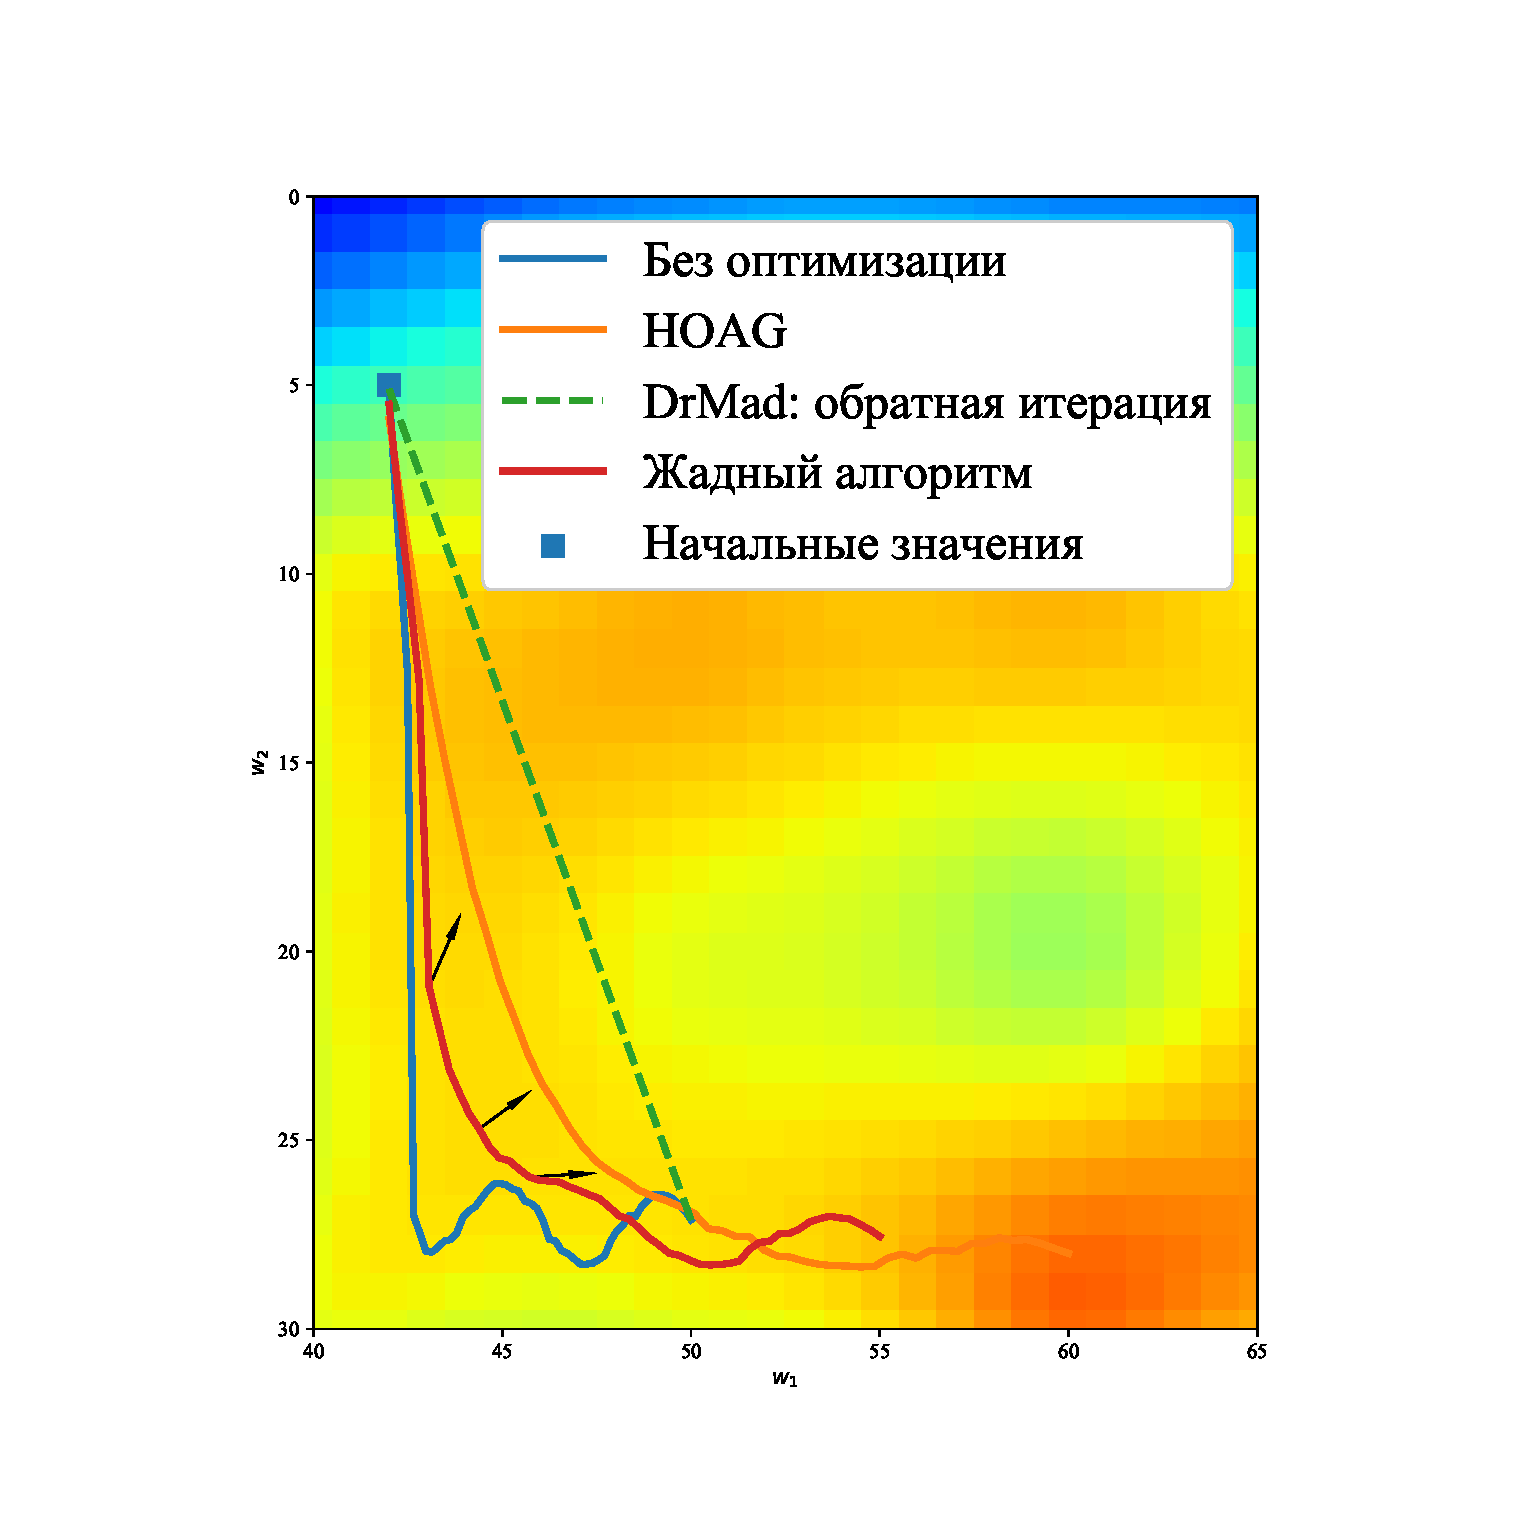
\includegraphics[width=0.6\linewidth]{plots/hyperparams/Fig_traj.eps}

    \caption{Иллюстративный пример действия операторов оптимизации на гиперпараметры. Интенсивность цвета графика соответствует значения функции валидации $Q$.}
 \label{fig:traj}
   
    \end{figure}




\section{Анализ алгоритмов оптимизации гиперпараметров}
Для анализа рассматриваемых алгоритмов оптимизации гиперпараметров был проведен ряд вычислительных экспериментов на выборках MNIST~\cite{mnist}, WISDM~\cite{wisdm}, а также на синтетических данных. Рассматривались задачи классификации и регрессии. В случае задач регрессии рассматриваемые модели $\mathbf{f}$ возвращали скалярные значения:
\[
    \mathbb{Y} \subset R, \quad \mathbf{f}(\mathbf{w}, \mathbf{x}) = f(\mathbf{w}, \mathbf{x}).
\]

Рассматривались следующие критерии качества:
\begin{enumerate}
\item Наилучшее значение $\hat{Q} = \max_{j \in \{1, \dots, l\}}Q^j$.
\item Среднее число итераций алгоритма для сходимости. Под данным показателем понимается число шагов оптимизациии гиперпараметров, при котором ошибка $Q$ изменяется не более чем на 1\% от своего наилучшего значения:
\[
    \argmin_{j}: \frac{Q^j - Q^0}{\hat{Q} - Q^0} \geq 0.99,
\]
где $Q^0$ --- значение функции $Q$ до начала оптимизации гиперпараметров.

\item Внешний критерий качества моделей $E$:
\[
    E = \text{RMSE} = \left (\frac{1}{m}\sum_{i=1}^m (f(\mathbf{x}_i, \mathbf{w})-y_i)\right)^{\frac{1}{2}}
\]
в случае задачи регрессии TODO: опять вопрос насчет меток,
\[
    E = \text{Accuracy} = 1 - \frac{1}{m}\sum_{i=1}^m [\argmax_{r \in \{1, \dots, R\}}f^r(\mathbf{x}_i, \mathbf{w}) \neq y_i]
\]
в случае задачи классификации.

\item Внешний критерий качества моделей $E_\sigma$ при возмущении параметров модели:
\[
    E_\sigma = \text{RMSE}_\sigma = \left (\frac{1}{m}\sum_{i=1}^m (f(\mathbf{x}_i, \mathbf{w} + \boldsymbol{\varepsilon})-y_i)\right)^{\frac{1}{2}}, \quad \boldsymbol{\varepsilon} \sim \mathcal{N}\bigl(\mathbf{0}, \sigma\mathbf{I}\bigr),
\]
\[
    E_\sigma  = \text{Accuracy}_\sigma  = 1 - \frac{1}{m}\sum_{i=1}^m [\argmax_{r \in \{1, \dots, R\}}f^r(\mathbf{x}_i, \mathbf{w }  + \boldsymbol{\varepsilon})) \neq y_i],  \quad \boldsymbol{\varepsilon} \sim \mathcal{N}\bigl(\mathbf{0}, \sigma\mathbf{I}\bigr).
\]

\end{enumerate}

%Для каждого алгоритма для синтетической выборки было проведено 50 повторений, результаты были усреднены. 
%Для остальных выборок было проведено 5 повторений. 
В качестве улучшаемого алгоритма рассматривался случайный поиск параметров с количеством итераций поиска, совпадающих с количеством итераций оптимизации гиперпараметров $l$: количество итераций $l=50$ для синтетической выборки и выборки WISDM, $l=25$ для выборки MNIST. В качестве функций $Q$ и $L$ рассматривались функции кросс-валидации~\eqref{eq:cv} с $k=4$ и вариацонная оценка обоснованности~\eqref{eq:hyper_elbo}. 




На всех выборках гиперпараметры инициализировались случайно из равномерного распределения:
\[
    \mathbf{h} \sim \mathcal{U}(a,b)^{|\mathbb{H}|},
\]
где $a = -2, b = 10$ для синтетической выборки и $a = -4, b = 10$ для выборок WISDM и MNIST.

Длина градиентного шага $ \lambda_{\text{lr}}^{\mathbf{h}}$ подбиралась для каждого алгоритма из сетки значений вида $\{r \cdot 10^{s}, s \leq 1, r \in \{1,25,50,75\}\}$  таким образом, чтобы итоговое значение гиперпараметров  $\mathbf{h}$  удовлетворяло следующему правилу:
\[
    a_\text{min} \leq  \min(\mathbf{h}), \quad \max(\mathbf{h}) \leq b_\text{max},
\] 
где  $a_\text{min} = -2.5, b_\text{max}=10.5$ для синтетической выборки и $a_\text{min} = -5, b_\text{max}=11$ для для выборок WISDM и MNIST.
Калибровка значения $ \lambda_{\text{lr}}$ проводилась на небольшом количестве итераций оптимизаций гиперпараметров $l$:
$l = 50$ для синтетической выборки,  $l=10$ для выборки WISDM $l=5$ для выборки MNIST. В случае, если алгоритмы показывали неустойчивую работу непосредственно во время запуска эксперимента (взрыв градиента или численное переполнение), то длина шага $ \lambda_{\text{lr}}^\mathbf{h}$ понижалась. Для алгоритма DrMad параметр $\tau_k$, отвечающий за количество рассматриваемых шагов оптимизации был установлен как $\tau_k=1$ для синтетической выборки и выборки WISDM, $\tau_k=10$ для выборки MNIST.



\textbf{Синтетическая выборка. }
Синтетические данные были порождены из выборки с одним признаком, $\mathbf{X} \in \mathbb{R}^{m \times 1}$.
Порождения выборки происходило по следующему правилу:
\[
	\mathbf{y} = \mathbf{X} + \boldsymbol{\varepsilon},\quad \mathbf{X}  \sim \mathcal{N}(\mathbf{0}, \mathbf{I}) \quad \boldsymbol{\varepsilon} \sim \mathcal{N}(\mathbf{0}, \mathbf{I}),
\]
где $\quad m = 40.$
В качестве модели $\mathbf{f}$ выступает регрессия с признаками $\{\mathbf{X}^0, \dots, \mathbf{X}^9, \textbf{sin}(\mathbf{X}), \textbf{cos}(\mathbf{X})\}$.

Было проведено 5 запусков для каждого алгоритма.
Графики итоговых полиномов представлены на Рис.~\ref{fig:poly}. Как видно из графиков, с использованием вариационной оценки удалось получить полиномы, близкие к линейным моделям. Подобные модели показывают наилучшее значение обоснованности в силу слабого переобучения и хорошего качества на тестовой выборке. 


\textbf{WISDM. }
Выборка WISDM состоит из набора записей акселерометра. Каждой записи соответствуют три координаты по осям акселерометра. В качестве набора объектов рассматривалось наборы из 199 последовательных записей акселерометра. В качестве набора меток рассматривалась евклидовая норма соответствующих 200-х записей акселерометра.

Рассматривалась нейросеть с 10 нейронами на скрытом слое:
\[
    \mathbf{f} = \mathbf{w}_2 \cdot \textbf{relu}(\mathbf{w}_1\mathbf{X} + \mathbf{b}_1) +\mathbf{b}_2,
\]
где $\mathbf{w}_1, \mathbf{b}_1$ --- параметры первого слоя нейросети,
$\mathbf{w}_2, \mathbf{b}_2$ --- параметры второго слоя нейросети,
\[
    \textbf{relu}(\mathbf{x}) = \textbf{max}(\mathbf{0}, \mathbf{x}).
\]

Графики сходимости алгоритмов, а также качества полученных моделей представлены на Рис.~\ref{fig:wisdm}.
Как видно из графиков, градиентные алгоритмы DrMad и HOAG показывают значительно худший результат по сравнению с жадным алгоритмом оптимизации. Случайный поиск показыват достаточно хорошие результаты в случае небольшого числа оптимизируемых гиперпараметров $\mathbf{h}$. В случае, когда в качестве функции $Q$ используется вариационная нижняя оценка обоснованности~\eqref{eq:hyper_elbo} и количество гиперпараметров велико, эффективно работающими алгоритмами оказалась жадная оптимизация и HOAG. HOAG имеет большее время сходимости и требует более сложных вычислений в процессе оптимизации.


\textbf{MNIST. }
Выборка MNIST состоит из множества изображений рукописных цифр.
Рассматривалась нейросеть с 300 нейронами на скрытом слое.

Графики сходимости алгоритмов, а также качества полученных моделей представлены на Рис.~\ref{fig:mnist}.
Как видно из графиков, модели, достигающиие наилучшей оценки обоснованности, имеют наихудшее итоговое качество, но более устойчивы к возмущению параметров модели. Для дополнительного анализа данной проблемы были проведены эксперименты по оптимизации моделей на выборке с добавленным шумом и использованием значений гиперпараметров $\mathbf{h}$, полученных ранее:
\[
    \hat{\mathfrak{D}} = \mathfrak{D} + \boldsymbol{\varepsilon}, \quad   \boldsymbol{\varepsilon} \sim \mathcal{N}(\mathbf{0}, \hat{\sigma}\mathbf{I}),
\]
где $\hat{\sigma}$ варьировалась в отрезке от 0 до 0.5.
График зависимости качества моделей от значения $\hat{\sigma}$ приведен на Рис.~\ref{fig:noise}.  Гиперпараметры, достигающие наибольших значений вариационной оценки~\eqref{eq:hyper_elbo} менее подвережены шуму в обучающей выборке, что можно интерпретировать как меньшую подверженность к переобучению.

Как можно видеть по результатам экспериментов, градиентные методы показывают лучший результат, чем случай поиск в случае большого количество гиперпараметров. Наилучшие результаты были получены жадным поиском. Алгоритм DrMad, показавший результаты хуже, чем жадный алгоритм и HOAG, является упрощенной версией алгоритма, представленного в~\cite{hyper_mad}. Данный алгоритм позволяет проводить оптимизацию не только гиперпараметров, но параметров алгоритма оптимизации $T$. Поэтому возможным развитием  метода DrMad является получение оптимальных значений параметров оптимизации.


\begin{table}
\small
\begin{tabularx}{\textwidth}{ |X|X|X|X|X|X|X|X|X|}

\hline
\textbf{Algorithm} & $L, Q$  & $Q(\mathbf{h}| \boldsymbol{\theta} )$ & Convergence & E & $E_{0.25}$ & $E_{0.5}$\\ 
\hline
\multicolumn{7}{|c|}{\textit{Synthetic}}  \\
\hline
Random search & ~\eqref{eq:cv} & \bf -171.6  &\bf 26.2 $\pm$ 20.0  & \bf 1.367 &\bf 1.410 &\bf 1.555 \\
\hline
Greedy & ~\eqref{eq:cv} & -172.5 & 30.0 $\pm$ 24.5 & 1.421 & 1.439 &  1.536\\
\hline
DrMAD & ~\eqref{eq:cv} & -174.1 & 40.2 $\pm$ 16.1 &  1.403 & 1.424 & \bf 1.512 \\
\hline
HOAG & ~\eqref{eq:cv} &-174.7 & 29.4 $\pm$ 24.0 &   \bf 1.432  & 1.463 & 1.553\\
\hline
Random Search & ~\eqref{eq:hyper_elbo} & -63.5  & 32.4 $\pm$ 18.7  & 1.368 & 1.426 & 1.546  \\
\hline
Greedy & ~\eqref{eq:hyper_elbo} & -25.5 & \bf 1.2 $\pm$ 0.4 & 1.161 & 1.174 & 1.193\\
\hline
DrMAD & ~\eqref{eq:hyper_elbo} & \bf -25.1 &  10.6 $\pm$ 0.8 &  1.157 & 1.163 &  1.184\\
\hline
HOAG & ~\eqref{eq:hyper_elbo} &-25.8 & 10.8 $\pm$ 1.5&   \bf 1.141  & \bf 1.149 & \bf 1.177\\
\hline


\multicolumn{7}{|c|}{\textit{WISDM}}  \\
\hline
Random search & ~\eqref{eq:cv} & \bf -1086661.1  & 22.0 $\pm$ 19.3  & \bf 0.660 & \bf 0.670 & \bf 0.690  \\
\hline
Greedy & ~\eqref{eq:cv} & -1086707.1 & \bf 15.4 $\pm$ 17.2 & 0.707 &  0.723  &  0.769\\
\hline
DrMAD & ~\eqref{eq:cv} & -1086708.2 & 29.2 $\pm$ 8.0 &  0.694 &  0.708 & 0.742 \\
\hline
HOAG & ~\eqref{eq:cv} & -1086733.5 & 28.2 $\pm$ 7.13&   0.701 & 0.724 & 0.753 \\
\hline
Random search & ~\eqref{eq:hyper_elbo} & -35420.4 &   14.4 $\pm$ 7.8  &   0.732 &   0.755 & 0.785 \\
\hline
Greedy & ~\eqref{eq:hyper_elbo} & \bf -3552.9 &\bf 1.0 $\pm$ 0.0  &   \bf 0.702 & \bf 0.730  &  \bf 0.767\\
\hline
DrMAD & ~\eqref{eq:hyper_elbo} & -26091.4 &   50.0 $\pm$ 0.0  & 0.729 &  0.753 & 0.816 \\
\hline
HOAG & ~\eqref{eq:hyper_elbo} &  -16566.6 & 49.0 $\pm$ 0.0  &  0.733 &  0.755 &  0.801 \\
\hline



\multicolumn{7}{|c|}{\textit{MNIST}}  \\
\hline
Random search & ~\eqref{eq:cv} & -3236.4  & 7.8 $\pm$ 1.9  &   0.981 & \bf 0.966 & \bf 0.866 \\
\hline
Greedy & ~\eqref{eq:cv} & \bf -3416.7 & 10.8 $\pm$ 10.4 & 0.979 & 0.962 & 0.860\\
\hline
DrMAD & ~\eqref{eq:cv} & -3469.0 & 17.0 $\pm$ 5.6 & \bf  0.982 & 0.962 & 0.831\\
\hline
HOAG & ~\eqref{eq:cv} & -3748.6 & \bf 8.6 $\pm$ 7.3&   0.980 &  0.961  & 0.853 \\
\hline
Random search & ~\eqref{eq:hyper_elbo} & -1304556.4 &  14.2 $\pm$ 5.7 &  \bf 0.982 & 0.943 & 0.814 \\
\hline
Greedy & ~\eqref{eq:hyper_elbo} & \bf -11136.2 & \bf 1.0 $\pm$ 0.0  &  0.977 & \bf 0.952 & \bf 0.884\\
\hline
DrMAD & ~\eqref{eq:hyper_elbo} & -1305432.9 & 24.6 $\pm$ 0.5  & \bf 0.982 & 0.941 & 0.813 \\
\hline
HOAG & ~\eqref{eq:hyper_elbo} &  -280061.6 & 24.0 $\pm$ 0.0  & 0.981 & 0.943 & 0.819\\
\hline


\hline
\end{tabularx}
\caption{Experiment results}
\label{table:table}
\end{table}


    \begin{figure}
     \begin{minipage}[t]{.5\textwidth}
    
    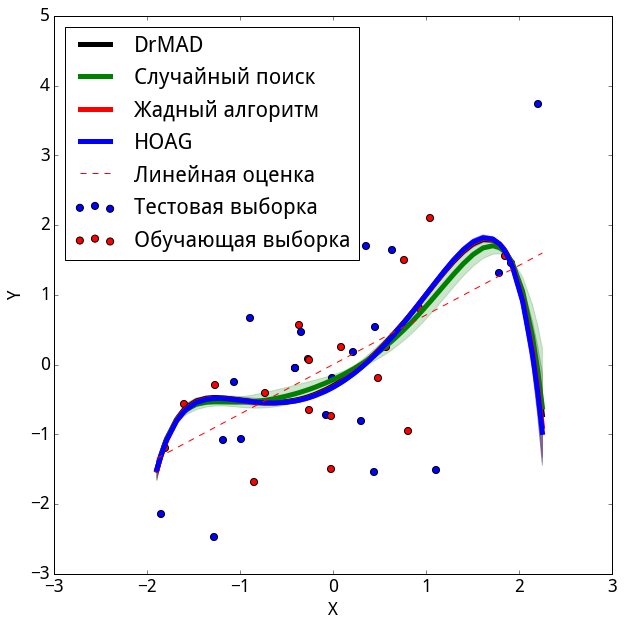
\includegraphics[width=\linewidth]{plots/hyperparams/poly_cv.png}
    \subcaption{}
    \end{minipage}
     \begin{minipage}[t]{.5\textwidth}
    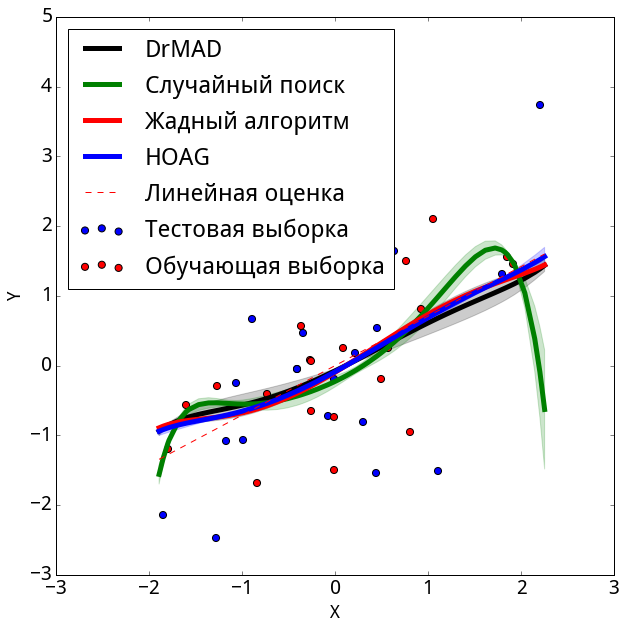
\includegraphics[width=\linewidth]{plots/hyperparams/poly_var.png}
    \subcaption{}   
\end{minipage}
    
 \caption{Итоговые модели для синтетической выборки: а) с использованием кросс-валидации, б) с использованием вариационной оценки обоснованности модели.}
  \label{fig:poly}
   
    \end{figure}




    \begin{figure}

    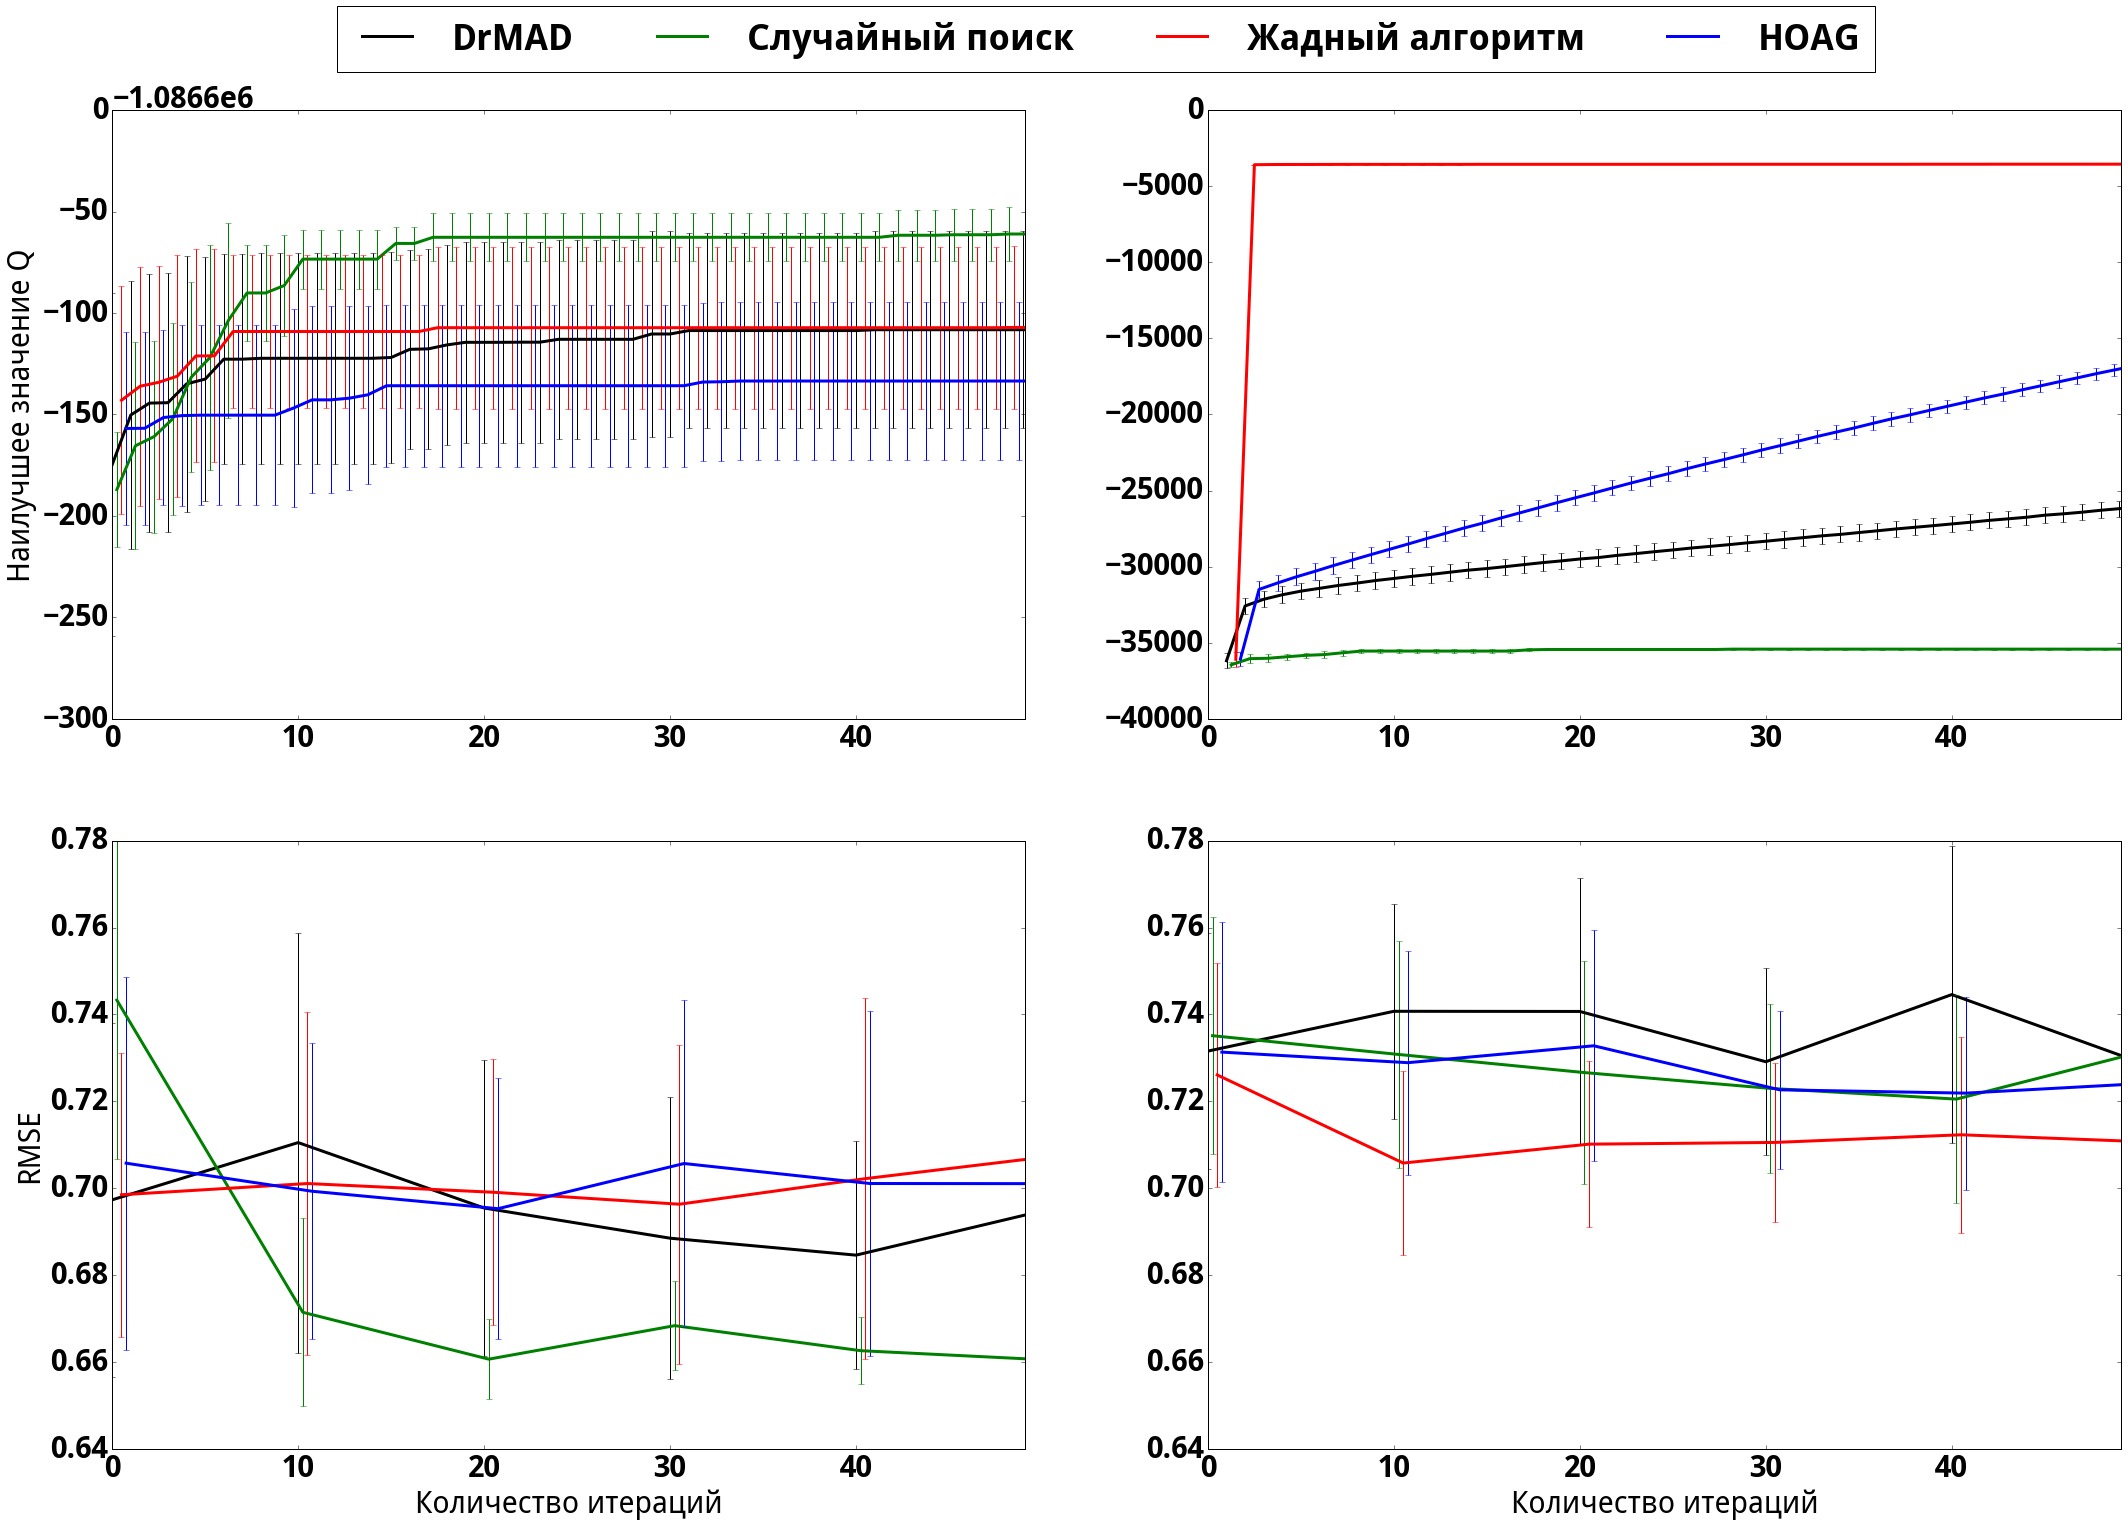
\includegraphics[width=\linewidth]{plots/hyperparams/wisdm.png}
\caption{WISDM,  наилучшее значение функции $Q$ и RMSE   для кросс-валидации (слева) и вариационной оценки обоснованности модели (справа).}    
\label{fig:wisdm}
    
    \end{figure}


    \begin{figure}

    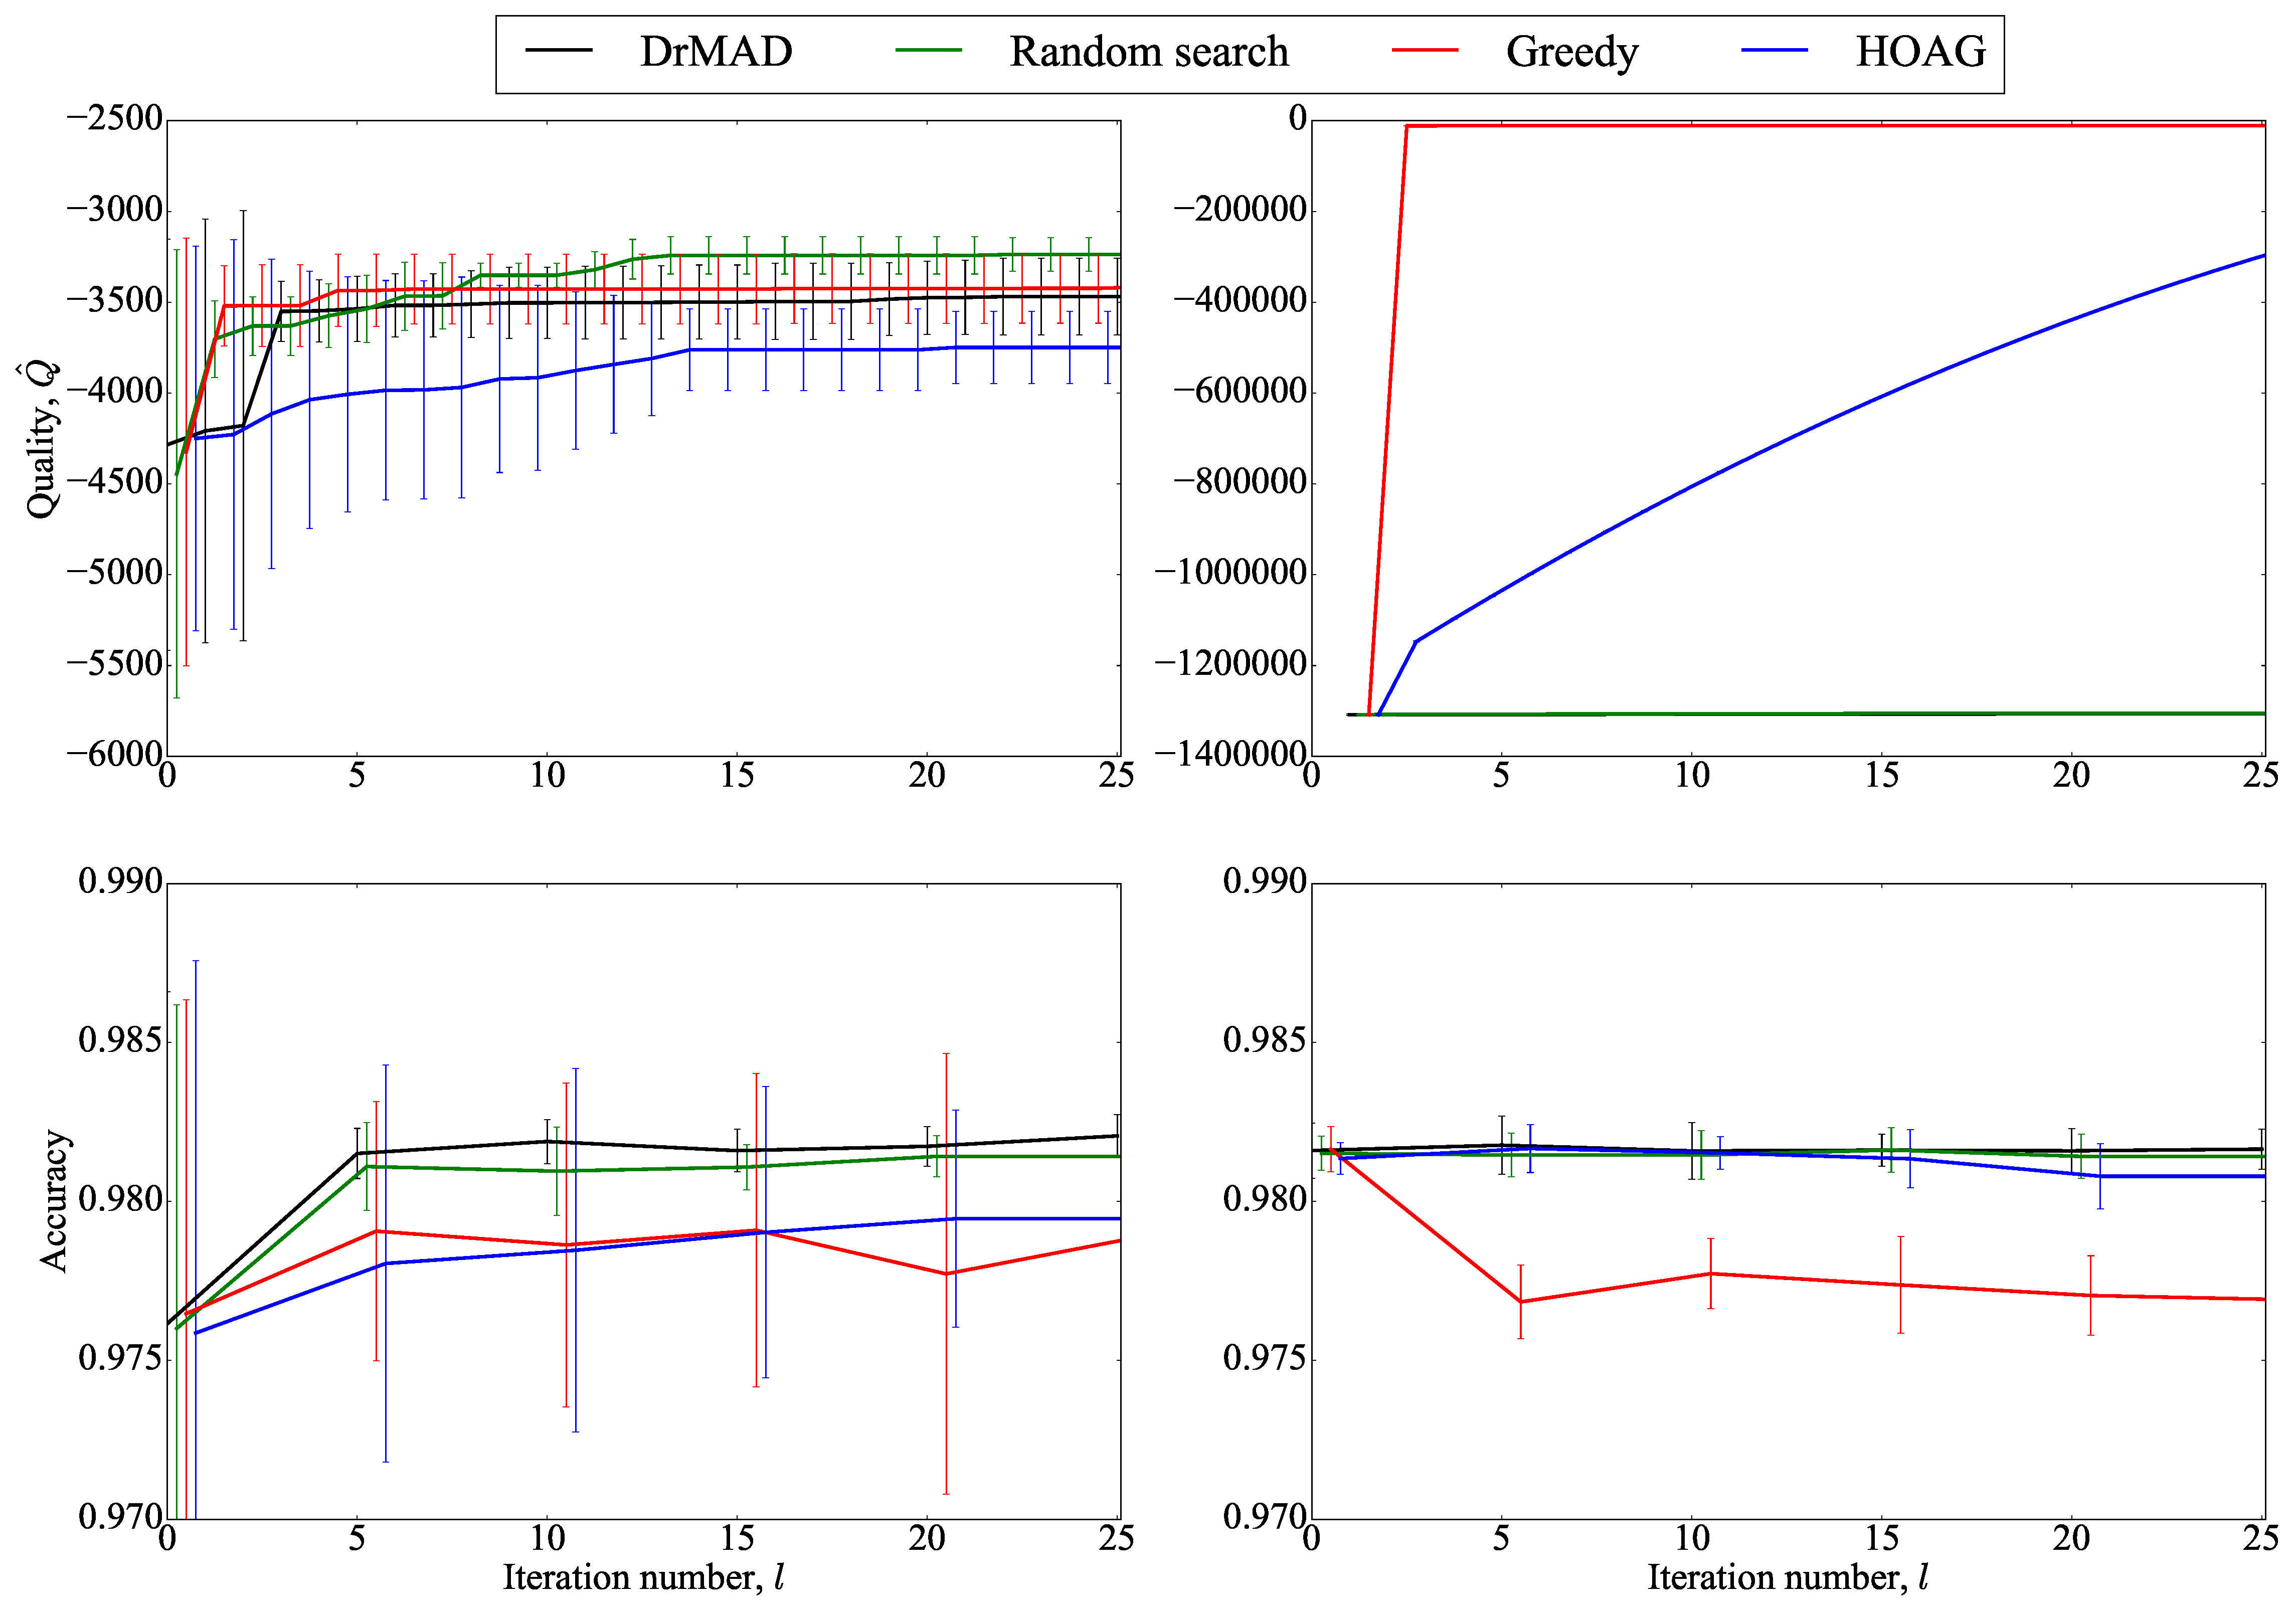
\includegraphics[width=\linewidth]{plots/hyperparams/Fig_mnist.eps}

    \caption{MNIST, наилучшее значение функции $Q$ и RMSE   для кросс-валидации (слева) и вариационной оценки обоснованности модели (справа).}
    \label{fig:mnist}
    \end{figure}

    \begin{figure}

    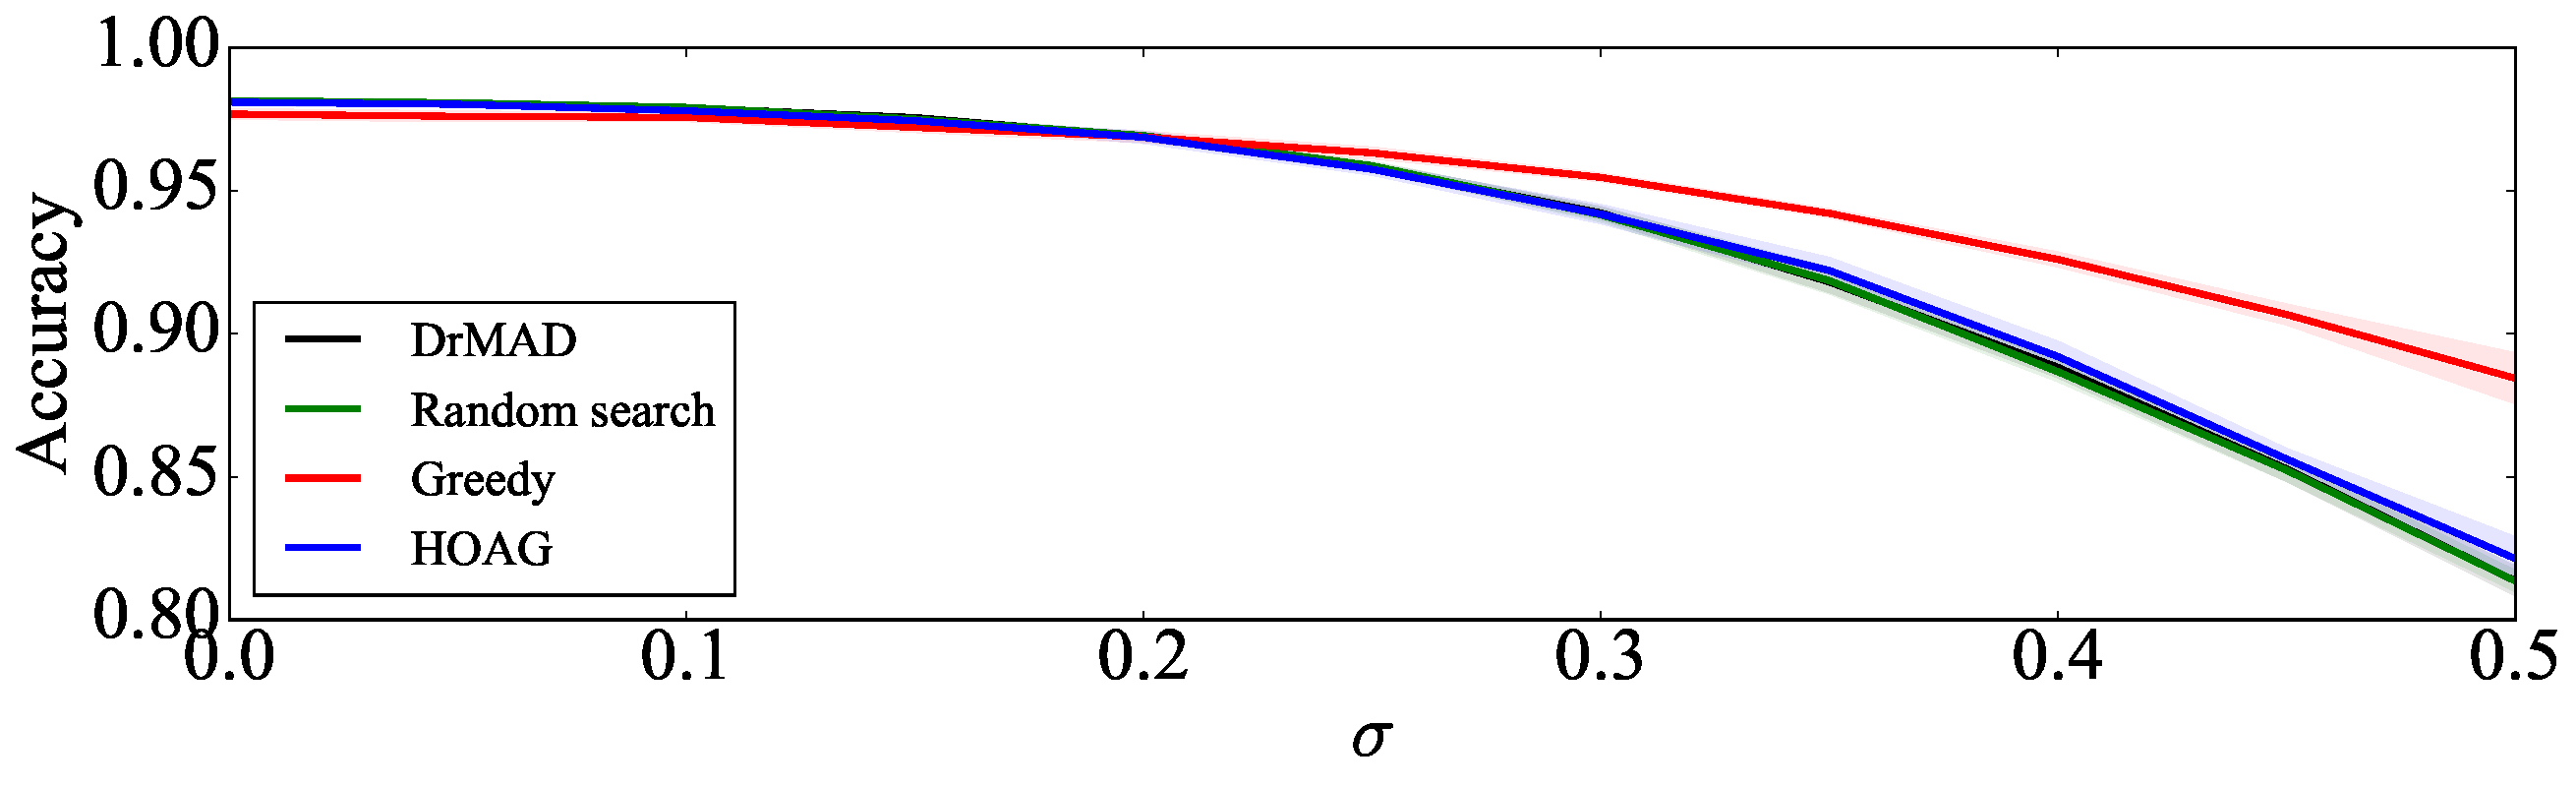
\includegraphics[width=\linewidth]{plots/hyperparams/Fig_noise.pdf}

    \caption{MNIST, точность классификации на тестовой выборке при добавлении шума в обучающую выборку. Гиперпараметры был оптимизированы с использованием вариационной оценки обоснованности модели.}
    \label{fig:noise}
    \end{figure}






